\documentclass[
,hyperref={pdfpagelabels=false}
]{beamer}
% Die Hyperref Option hyperref={pdfpagelabels=false} verhindert die Warnung:
% Package hyperref Warning: Option `pdfpagelabels' is turned off
% (hyperref)                because \thepage is undefined.
% Hyperref stopped early

\usepackage{agstyle}
\usepackage{currycode}
\usepackage{tikz}

\newcommand{\ergo}{$\Rightarrow$}

%%%%%%%%%%%%%%%%%%%%%%%%%%%%%%%%%%%%%%%%%%%%%%%%%%%%%%%%%%%%%%%%%%%%%%%%%%%%%%%%

\title[Handling Non-Determinism in KiCS2]{%
Handling Non-Determinism in KiCS2: \\ More than just searching?
}

\date{February 01, 2012}

\author[Braßel, Hanus, \underline{Peemöller}, Reck]{%
\texorpdfstring
  {Bernd Braßel \and Michael Hanus \\
   \underline{Björn Peemöller} \and Fabian Reck}
  {Bernd Braßel \and Michael Hanus \and Björn Peemöller \and Fabian Reck}
}

\institute{Kiel University}

\begin{document}

\begin{frame}%---------------
\titlepage
\end{frame}

%%%%%%%%%%%%%%%%%%%%%%%%%%%%%%%%%%%%%%%%%%%%%%%%%%%%%%%%%%%%%%%%%%%%%%%%%%%%%%$$

\section{Introduction}

\begin{frame}[fragile]
\frametitle{Previously on KiCS2}
\begin{itemize}
\item KiCS2 is a compiler from Curry to Haskell
\item Non-determinism is explicitly represented in
      the data structures
\item Unique identifiers are used to obtain
      call-time choice semantics
\item Optimizations for deterministic and higher order functions
\end{itemize}
\end{frame}

%%%%%%%%%%%%%%%%%%%%%%%%%%%%%%%%%%%%%%%%%%%%%%%%%%%%%%%%%%%%%%%%%%%%%%%%%%%%%%

\section{Runtime Representations}

\begin{frame}[fragile]%-------------------------------------------------------
\frametitle{Runtime Representation of Choice}
\begin{itemize}
  \item Explicit representation of non-determinism in data types
  \item Choices are uniquely identified
\end{itemize}

\begin{curry}
data Bool = True | False

aBool :: Bool
aBool = True ? False
\end{curry}

\begin{haskell}
data Bool = True | False | Choice ID Bool Bool

aBool :: IDSupply -> Bool
aBool s = Choice (thisID s) True False
\end{haskell}
\end{frame}

\begin{frame}[fragile]%-------------------------------------------------------
\frametitle{Identifying Choices}
\begin{itemize}
 \item \code{ID}s are provided by an \code{IDSupply}
       (infinite set of \code{ID}s)
 \item \code{IDSupply}s can be split into disjoint subsets
 \item Functions that may introduce non-determinism
       are provided with an \code{IDSupply}
\end{itemize}

\begin{haskell} [Choice Identifiers using Integer]
type ID = Integer
type IDSupply = Integer

left, right :: IDSupply -> IDSupply
left  n = 2 * n
right n = 2 * n + 1

thisID :: IDSupply -> ID
thisID n = n
\end{haskell}
\end{frame}

\begin{frame}[fragile]%-------------------------------------------------------
\frametitle{Representing Failure}
\begin{itemize}
 \item Computing with failure is a common programming pattern in FLP
 \item Failures do not abort the computation
\end{itemize}

\begin{curry}
ensureTrue True = True
\end{curry}

\begin{haskell}
data Bool = True | False | Choice ID Bool Bool \alert{| Fail}

ensureTrue True             = True
ensureTrue (Choice i x1 x2) = Choice i (ensureTrue x1)
                                       (ensureTrue x2)
\alert{ensureTrue _                = Fail}
\end{haskell}
\end{frame}

% \begin{frame}[fragile]%-------------------------------------------------------
% \frametitle{Representing Free Variables}
%
% \begin{itemize}
%  \item Idea: Free Variables non-deterministically generate every value
%        of the respective type
%  \item $n$-ary constructor \code{Choices} instead of nested
%        \code{Choice}s to allow constructors to share the same level
% \end{itemize}
%
% \begin{curry}
% aBool :: Bool
% aBool = x where x free
%
% aList :: [Bool]
% aList = xs where xs free
% \end{curry}
%
% \begin{haskell}
% aBool :: IDSupply -> Bool
% aBool s = Choices (thisID s) [True, False]
%
% aList :: IDSupply -> [Bool]
% aList s = Choices (thisID s) [[], aBool (left s) : aList (right s)]
% \end{haskell}
% \end{frame}

\begin{frame}[fragile]%-------------------------------------------------------
\frametitle{Normalform computation}
\begin{itemize}
%   \item Non-determinism in arguments is propagated by pattern-matching
  \item Constructors may be applied to non-deterministic arguments
  \item \code{normalform} traverses a constructor term
        to propagate non-determinism
  \item After normalform computation of an expression $e$
  \begin{itemize}
    \item \code{normalform e} is either a deterministic value
    \item or a tree, where the inner nodes correspond to \code{Choice} or
          \code{Choices} and all leafs are either \code{Fail} or
          deterministic values
  \end{itemize}
\end{itemize}

\pause

\begin{example}[Normalform Computation of \code{(\textbackslash x -> (x,x)) (0 ? 1)}]
\begin{center}
\begin{minipage}{.2\textwidth}
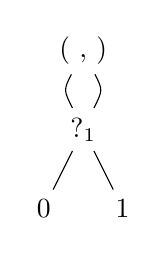
\begin{tikzpicture}
\node (t) at (0  ,0) {\code{0}};
\node (f) at (1  ,0) {\code{1}};
\node (q) at (0.5,1) {$\code{?}_{1}$};
\node (l) at (0.5,2) {\code{( , )}};
\draw (l) .. controls (0.25,1.5) .. (q);
\draw (l) .. controls (0.75,1.5) .. (q);
\draw (q) -- (t);
\draw (q) -- (f);
\end{tikzpicture}
\end{minipage}
$\Rightarrow$
\begin{minipage}{.2\textwidth}
\begin{tikzpicture}
\node (t ) at (0  ,0) {\code{0}};
\node (f ) at (1  ,0) {\code{1}};
\node (q1) at (0.5,1) {$\code{?}_{1}$};
\node (v1) at (0  ,2) {\code{(0, )}};
\node (v2) at (1  ,2) {\code{(1, )}};
\node (q2) at (0.5,3) {$\code{?}_{1}$};
\draw (q2) -- (v1);
\draw (q2) -- (v2);
\draw (v1) -- (q1);
\draw (v2) -- (q1);
\draw (q1) -- (t);
\draw (q1) -- (f);
\end{tikzpicture}
\end{minipage}
$\Rightarrow$
\begin{minipage}{.36\textwidth}
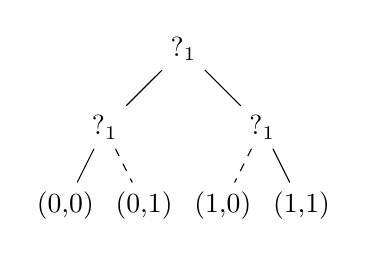
\begin{tikzpicture}
\node (tt) at (0  ,0) {\code{(0,0)}};
\node (tf) at (1  ,0) {\code{(0,1)}};
\node (ft) at (2  ,0) {\code{(1,0)}};
\node (ff) at (3  ,0) {\code{(1,1)}};
\node (q1) at (0.5,1) {$\code{?}_{1}$};
\node (q2) at (2.5,1) {$\code{?}_{1}$};
\node (q3) at (1.5,2) {$\code{?}_{1}$};
\draw (q3) -- (q1);
\draw (q3) -- (q2);
\draw (q1) -- (tt);
\draw[style=dashed] (q1) -- (tf);
\draw[style=dashed] (q2) -- (ft);
\draw (q2) -- (ff);
\end{tikzpicture}
\end{minipage}
\end{center}
\end{example}
\end{frame}


%%%%%%%%%%%%%%%%%%%%%%%%%%%%%%%%%%%%%%%%%%%%%%%%%%%%%%%%%%%%%%%%%%%%%%%%%%%%%%

\section{Search}

\begin{frame}[fragile]%-------------------------------------------------------
\frametitle{Top-Level Search}

\begin{itemize}
  \item Implemented in the \code{IO} monad
  \item Global decision store
  \item One implementation per strategy, fastest for dfs
\end{itemize}

\begin{haskell}[Depth-first-search]
dfs :: Try a -> IO ()
dfs (Val a)        = print a
dfs Fail           = return ()
dfs (Choice i l r) = lookupDecision i >>= follow
  where
  follow ChooseLeft  = dfs (try l)
  follow ChooseRight = dfs (try r)
  follow NoDecision  = do decide i ChooseLeft  l
                          decide i ChooseRight r

  decide i c x = do setDecision i c >> dfs (try x)
                    setDecision i NoDecision
\end{haskell}
\end{frame}

\begin{frame}[fragile]%-------------------------------------------------------
\frametitle{Managing Decisions}
\begin{itemize}
\item During search, consistent decisions have to be made
\item Management of decisions is abstracted by a type class
\end{itemize}

\begin{haskell}[Search decisions]
data Decision = NoDecision
              | ChooseLeft
              | ChooseRight

class Monad m => Store m where
  lookupDecision :: ID -> m Decision
  setDecision    :: ID -> Decision -> m ()
\end{haskell}
\end{frame}

\begin{frame}[fragile]%-------------------------------------------------------
\frametitle{Monadic Search}

\begin{itemize}
  \item Implemented using a \code{State} monad
  \item Local decision store
  \item Independent of search strategy
\end{itemize}

\begin{haskell}[General search]
search :: (MonadPlus m, Store m) => Try a -> m a
search (Val a)        = return a
search Fail           = mzero
search (Choice i l r) = lookupDecision i >>= follow
  where
  follow ChooseLeft  = search (try l)
  follow ChooseRight = search (try r)
  follow NoDecision  = decide i ChooseLeft  l
               `mplus` decide i ChooseRight r

  decide i c x = setDecision i c >> search (try x)
\end{haskell}
\end{frame}

\begin{frame}[fragile]%-------------------------------------------------------
\frametitle{Search strategies}
\begin{itemize}
  \item Based on tree representation of search space
  \item Strategies only extract values
  \item Available: depth-first, breadth-first, iterative deepening
\end{itemize}

\begin{haskell}[SearchTree]
data SearchTree a = None
                  | One a
                  | Choice (SearchTree a) (SearchTree a)
\end{haskell}

\begin{haskell}[Depth-first-search using SearchTree]
dfsSearch :: SearchTree a -> [a]
dfsSearch None         = []
dfsSearch (One      x) = [x]
dfsSearch (Choice x y) = dfsSearch x ++ dfsSearch y
\end{haskell}
\end{frame}

\begin{frame}%----------------------------------------------------------------
\frametitle{Benchmark: Non-Deterministic Permutation Sort}
Program: permutation sort of a list with 15 values
\begin{center}
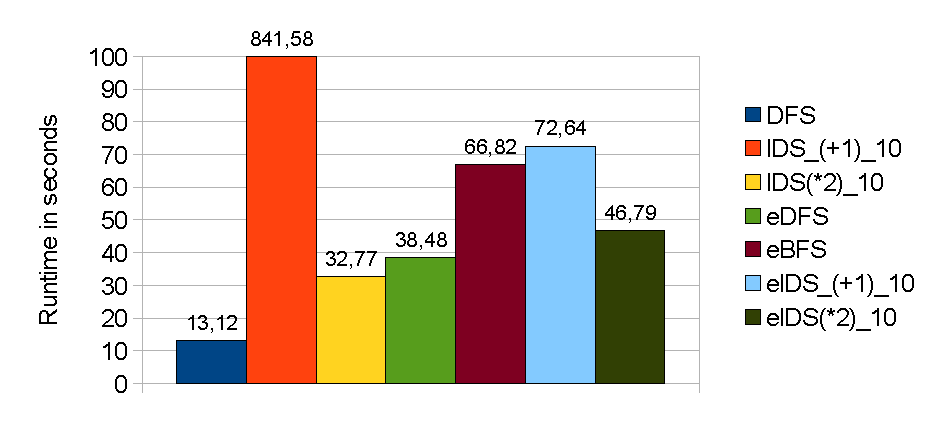
\includegraphics[width=11cm]{gfx/permsort}
\end{center}
\begin{itemize}
\item DFS is fastest
\item $\text{IDS}_{10}^{+1}$ is very slow due to the linear search space
\item $\text{eIDS}_{10}^{+1}$ profits from sharing the search tree
\end{itemize}
\end{frame}

% \begin{frame}[fragile]%-------------------------------------------------------
% \frametitle{Benchmark: Unification}
% Program: Compute the last element of a list by unification
% \begin{center}
% 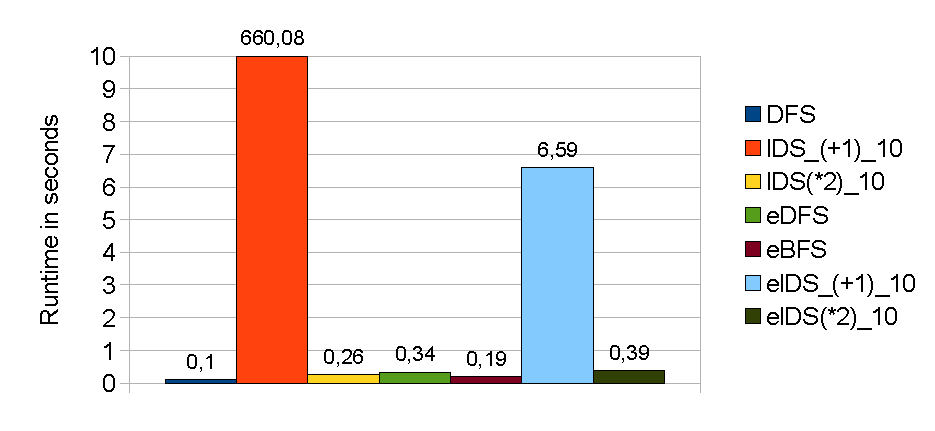
\includegraphics[width=11cm]{gfx/last}
% \end{center}
% \todo{Interpretation}
% \end{frame}

\begin{frame}[fragile]%-------------------------------------------------------
\frametitle{Benchmark: Halve a Peano Number}
Program: halve the Peano number $1600$ by inverting addition
\begin{center}
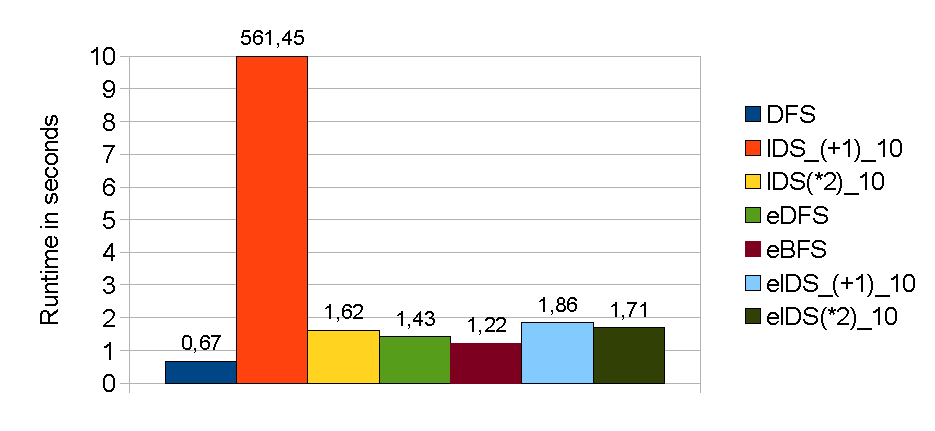
\includegraphics[width=11cm]{gfx/half}
\end{center}
\begin{itemize}
\item Again, DFS is fastest and $\text{IDS}_{10}^{+1}$ is very slow
\item Both encapsulated search as well as complete strategies are
      competitive
\end{itemize}
\end{frame}

%%%%%%%%%%%%%%%%%%%%%%%%%%%%%%%%%%%%%%%%%%%%%%%%%%%%%%%%%%%%%%%%%%%%%%%%%%%%%%

\begin{frame}[fragile]%-------------------------------------------------------
\frametitle{Encapsulated search}

\begin{itemize}
\item Top-Level search is not always sufficient (e.\,g., when trying to
      find the best solution)
\item \emph{Encapsulated search} allows to search for all values
      inside Curry
\item Implemented by providing a \code{MonadPlus} instance for the runtime
      representation of a search tree in Curry
\end{itemize}

\pause

\begin{curry}[Encapsulated dfs search]
allValuesDFS x = dfsSearch (someSearchTree x)
\end{curry}

\begin{example}[Encapsulated search]
\begin{program}
f x  = id x ? not x
bool = True ? False

> \textsl{allValuesDFS (f bool)}
[True,False,False,True]
\end{program}
\end{example}

\end{frame}

\begin{frame}[fragile]%-------------------------------------------------------
\frametitle{Set Functions}

\begin{itemize}
\item Encapsulated search is not independent of the evaluation order

\begin{program}
let x = 0 ? 1 in allValues (x ? -x)
\end{program}

\pause

\item Sharing of non-determinism is problematic w.r.t. encapsulated
      search

\begin{program}
queens xs | null (allValues (attack ys)) = ys
  where ys = permute xs
\end{program}

\pause

  \item[\ergo] \emph{Set functions} preserve non-determinism of arguments,
               but search for that introduced by the function itself
\end{itemize}

\begin{example}[Set Functions]
\begin{program}
f x = x ? -x
> \textsl{set_1 f (0 ? 1)}
\{0,0\}
\{1,-1\}
\end{program}
\end{example}

\end{frame}

\begin{frame}[fragile]%-------------------------------------------------------
\frametitle{Designated Implementation of Set Functions}

\begin{itemize}
  \item \code{ID}s can be covered to preserve non-determinism
  \item Search space representation needs to distinguish covered
        and uncovered non-determinism
  \item[\ergo] \code{MonadPlus} is extended to \code{MonadSearch}\footnote{%
       Better naming appreciated}
\end{itemize}

\pause

\begin{haskell}[Covered \code{ID}s]
data ID = ChoiceID  Int
        | CoveredID Int
\end{haskell}

\begin{haskell}[\code{MonadSearch}]
class MonadPlus m => MonadSearch m where
  splus :: ID ->  m a  -> m a -> m a -- preserve binary Choice
  ssum  :: ID -> [m a] -> m a        -- preserve n-ary  Choice
\end{haskell}

\end{frame}

%%%%%%%%%%%%%%%%%%%%%%%%%%%%%%%%%%%%%%%%%%%%%%%%%%%%%%%%%%%%%%%%%%%%%%%%%%%%%%

\section{Conclusion}

\begin{frame}[fragile]%-------------------------------------------------------
\frametitle{Conclusion}

\begin{itemize}
\item More flexibility of search
      \begin{itemize}
        \item Multiple search strategies
        \item Multiple levels to search non-determinism
      \end{itemize}
\item Applicability of search
      \begin{itemize}
        \item More than read-eval-print loop
        \item Non-determinism and I/O can be clearly separated
      \end{itemize}
\end{itemize}
\end{frame}

\end{document}
